\chapter{Métrique, expansion et premiers éléments de cosmologie}

À la fin du cours précédent, nous étions parvenus à une équation d’onde invariante de Lorentz et nous nous apprêtions à écrire les équations de Maxwell sous forme spatiotemporelle. Une question du public apporte maintenant un avertissement utile avant d’aborder la gravitation : dans quelle mesure la symétrie peut-elle déterminer à elle seule une théorie physique ? La réponse est sans équivoque : dans une large mesure, mais pas entièrement. L’invariance de Lorentz constitue un puissant filtre pour les lois possibles. Elle ne remplace ni les autres hypothèses physiques ni l’expérience.

\section{Ce que la symétrie ne détermine pas}

\begin{classroomqa}
\audiencequestion{Dès lors que l’on sait que les champs électrique et magnétique se transforment ensemble sous les transformations de Lorentz, les équations de Maxwell découlent-elles de la seule relativité ?}
\lecturerresponse{Non. La relativité contraint la forme des équations, mais leur construction fait aussi intervenir leur linéarité, le faible ordre de leurs dérivées, la manière dont les champs se transforment et des données expérimentales. Sans ces éléments supplémentaires, de nombreuses équations de champ covariantes de Lorentz resteraient possibles.}
\end{classroomqa}

La plus importante de ces hypothèses supplémentaires pour commencer est la linéarité. Si \(A(x,t)\) est une solution d’une équation de champ linéaire, alors \(\lambda A(x,t)\) est également une solution pour toute constante \(\lambda\). Si \(A\) et \(B\) sont des solutions, alors \begin{equation}
  C(x,t)=A(x,t)+B(x,t).
  \label{eq:superposition}
\end{equation}
C’est le principe de superposition. Deux ondes électromagnétiques sans source peuvent se croiser et ressortir inchangées. Elles n’entrent pas directement en collision comme le font des objets matériels. Elles peuvent interagir indirectement par l’intermédiaire de matière chargée, car chaque onde met les charges en mouvement et ces charges en mouvement rayonnent, mais les équations du champ dans le vide sont elles-mêmes linéaires.

\begin{figure}[H]
\centering
\includegraphics[width=0.64\textwidth]{lecture_08_figure_01.png}
\caption{Deux profils d’onde au tableau pendant la discussion sur la superposition. Leur somme est encore une onde sans source admissible.}
\lectureframe{00:05:30}
\end{figure}

L’oscillateur harmonique rend l’algèbre transparente. Supposons que \begin{equation}
  m\ddot x=-kx.
  \label{eq:linear-oscillator}
\end{equation}
Si \(x_1\) et \(x_2\) sont solutions de \eqref{eq:linear-oscillator}, alors \begin{equation}
  m(\ddot x_1+\ddot x_2)
  =-k(x_1+x_2),
\end{equation}
donc \(x_1+x_2\) est une solution. Ajoutons toutefois un terme non linéaire, \begin{equation}
  m\ddot x=-kx+p x^2,
  \label{eq:nonlinear-oscillator}
\end{equation}
et la somme ne convient plus :
\begin{equation}
  (x_1+x_2)^2=x_1^2+x_2^2+2x_1x_2.
\end{equation}
Le terme croisé \(2x_1x_2\) n’a pas d’équivalent dans les deux équations prises séparément. Les deux mouvements s’influencent désormais l’un l’autre.

\begin{figure}[H]
\centering
\includegraphics[width=0.73\textwidth]{lecture_08_figure_02.png}
\caption{Comparaison des équations de deux oscillateurs distincts avec l’équation de leur somme. Le terme quadratique fait apparaître le terme croisé supplémentaire qui rompt la superposition.}
\lectureframe{00:10:10}
\end{figure}

Cet exemple fixe le point méthodologique qui restera valable tout au long de la discussion sur la cosmologie. La symétrie nous indique quelles quantités peuvent être combinées et quelles équations sont admissibles. La dynamique et l’observation nous indiquent laquelle de ces équations admissibles la nature réalise.

\section{L’intervalle comme géométrie}

Nous quittons maintenant l’électromagnétisme pour emprunter une voie brève vers la relativité générale et la cosmologie. Le point de départ est l’intervalle entre deux événements voisins. Repérons un événement par les quatre coordonnées \(x^\mu\) et un événement proche par \(x^\mu+dx^\mu\). Dans des coordonnées cartésiennes inertielles, avec \(c=1\) et la convention \((+,-,-,-)\),
\begin{equation}
  d\tau^2
  =dt^2-dx^2-dy^2-dz^2
  =dx^\mu dx_\mu
  =\eta_{\mu\nu}\,dx^\mu dx^\nu.
  \label{eq:minkowski-interval}
\end{equation}
La quantité \(d\tau^2\), et non une différence de coordonnées particulière, est invariante. Les transformations de Lorentz modifient \(dt,dx,dy,dz\) tout en préservant cette combinaison quadratique. On peut donc comprendre la relativité restreinte comme la géométrie de l’espace-temps de Minkowski.

\begin{figure}[H]
\centering
\includegraphics[width=0.72\textwidth]{lecture_08_figure_03.png}
\caption{L’intervalle de Minkowski écrit successivement en notation par composantes, à indices contractés et avec le tenseur métrique.}
\lectureframe{00:14:50}
\end{figure}

La simplicité de \eqref{eq:minkowski-interval} dépend des coordonnées. Même un plan plat peut se voir attribuer des coefficients inhabituels si l’on choisit mal ses coordonnées. Supposons que \(x\) soit mesuré en centimètres tandis que \(y\) l’est en mètres. Pour un déplacement physique,
\begin{equation}
  ds^2=dx^2+\left(\frac{dy}{100}\right)^2
      =dx^2+10^{-4}dy^2.
  \label{eq:mixed-units}
\end{equation}
Le facteur \(10^{-4}\) ne dit rien sur la courbure. Il traduit simplement un changement d’unités.

\begin{figure}[H]
\centering
\includegraphics[width=0.59\textwidth]{lecture_08_figure_04.png}
\caption{Un plan plat décrit avec des centimètres sur un axe et des mètres sur l’autre. Les coefficients métriques inégaux encodent les unités, pas la courbure.}
\lectureframe{00:20:10}
\end{figure}

Des coordonnées obliques introduisent un terme mixte. En deux dimensions, la forme quadratique locale la plus générale peut s’écrire
\begin{align}
  ds^2
  &=a_{11}\,dx^2+a_{12}\,dx\,dy\notag\\
  &\quad+a_{21}\,dy\,dx+a_{22}\,dy^2,
  \qquad a_{12}=a_{21}.
  \label{eq:quadratic-form}
\end{align}
Comme les différentielles ordinaires commutent, \(dx\,dy=dy\,dx\), seule la partie symétrique du tableau des coefficients contribue. Regroupons les coefficients dans la matrice
\begin{equation}
  g=
  \begin{pmatrix}
    a_{11} & a_{12}\\
    a_{21} & a_{22}
  \end{pmatrix}.
  \label{eq:metric-matrix}
\end{equation}
Cette matrice est la \emph{métrique}. Elle donne la règle locale qui convertit les différences de coordonnées en intervalles physiques.

\begin{figure}[H]
\centering
\includegraphics[width=0.71\textwidth]{lecture_08_figure_05.png}
\caption{La forme quadratique différentielle et sa matrice des coefficients symétrique \(2\times2\) au moment où cette matrice est identifiée à la métrique.}
\lectureframe{00:24:07}
\end{figure}

Les grilles rectangulaires ou obliques uniformes donnent des coefficients constants. Si les lignes de coordonnées sont courbes, se resserrent ou s’écartent, ces coefficients deviennent des fonctions de la position, même si la surface sous-jacente reste plate. La notation générale de l’espace-temps est
\begin{equation}
  ds^2=g_{\mu\nu}(x)\,dx^\mu dx^\nu.
  \label{eq:general-metric}
\end{equation}

\begin{figure}[H]
\centering
\includegraphics[width=0.66\textwidth]{lecture_08_figure_06.png}
\caption{La métrique générale dépendant de la position, une fois que la grille de coordonnées peut varier d’un point à l’autre.}
\lectureframe{00:28:10}
\end{figure}

Connaître \(g_{\mu\nu}\) dans un système de coordonnées donné détermine les distances, les durées et les angles locaux, et donc la géométrie. La réciproque n’est pas unique : une même géométrie admet une infinité de descriptions en coordonnées, donc une infinité de tableaux de fonctions de coefficients reliés par des transformations de coordonnées.

\section{Complexité des coordonnées et courbure intrinsèque}

Nous devons maintenant distinguer une métrique compliquée d’un espace courbe. Enroulons une feuille de papier en cylindre sans l’étirer. Son apparence dans la pièce change, mais toutes les distances mesurées sur la feuille restent les mêmes. Une créature confinée au papier ne peut détecter cette déformation par aucune mesure intrinsèque. Il s’agit d’une déformation extrinsèque, et non de la courbure dont il est question ici.

Une hémisphère, c’est différent. On ne peut pas l’aplatir sans l’étirer, la déchirer ou la comprimer. Une carte plane de la Terre doit déformer les distances, les aires, les angles, ou une combinaison de ces éléments. Cet obstacle est intrinsèque et peut être détecté sans regarder dans une dimension environnante.

Les coordonnées polaires fournissent le contre-exemple plat indispensable. Dans un plan, un déplacement radial infinitésimal a pour longueur \(dr\), tandis qu’un déplacement angulaire \(d\theta\) à la distance radiale \(r\) a pour longueur \(r\,d\theta\). Ainsi,
\begin{equation}
  ds^2=dr^2+r^2d\theta^2,
  \qquad
  g_{\text{polar}}=
  \begin{pmatrix}
    1&0\\
    0&r^2
  \end{pmatrix}.
  \label{eq:polar-metric}
\end{equation}
Le coefficient \(r^2\) varie dans le plan, et pourtant celui-ci est plat. Le changement de variables
\begin{equation}
  x=r\cos\theta,\qquad y=r\sin\theta
\end{equation}
ramène la métrique constante \(ds^2=dx^2+dy^2\).

\begin{figure}[H]
\centering
\includegraphics[width=0.70\textwidth]{lecture_08_figure_07.png}
\caption{La métrique polaire et son retour à la métrique cartésienne. La matrice dépendant de la position à gauche décrit tout de même un plan plat.}
\lectureframe{00:39:20}
\end{figure}

\begin{classroomqa}
\audiencequestion{La distance angulaire en coordonnées polaires doit-elle comporter un sinus ?}
\lecturerresponse{Pas dans le plan. L’élément de longueur d’arc y vaut \(r\,d\theta\). Un sinus apparaît sur la sphère, où un cercle de latitude a pour rayon \(R\sin\theta\).}
\end{classroomqa}

Considérons une sphère de rayon \(R\). Soit \(\theta\) l’angle polaire mesuré depuis le pôle Nord et \(\phi\) l’angle azimutal. Un déplacement le long d’un méridien a pour longueur \(R\,d\theta\). À l’angle polaire \(\theta\), le cercle de latitude a pour rayon \(R\sin\theta\), de sorte qu’un déplacement azimutal a pour longueur \(R\sin\theta\,d\phi\). Le théorème de Pythagore local donne
\begin{align}
  ds^2
  &=R^2\left(d\theta^2+\sin^2\theta\,d\phi^2\right),
  \label{eq:sphere-metric}\\
  g_{\text{sphere}}=
  &\begin{pmatrix}
    R^2&0\\
    0&R^2\sin^2\theta
  \end{pmatrix}.
\end{align}

\begin{figure}[H]
\centering
\includegraphics[width=0.72\textwidth]{lecture_08_figure_08.png}
\caption{La sphère, son élément de ligne angulaire et la matrice métrique correspondante. Le facteur \(\sin^2\theta\) rend compte du rétrécissement des cercles de latitude.}
\lectureframe{00:45:15}
\end{figure}

\begin{figure}[H]
\centering
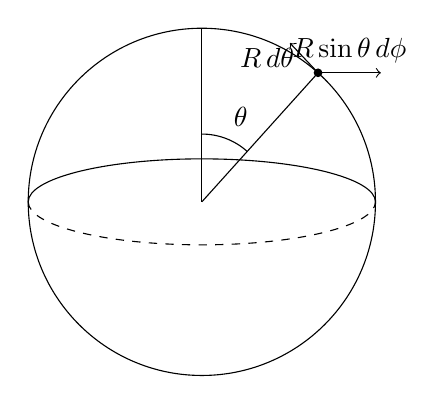
\begin{tikzpicture}[scale=1.05]
  \draw (0,0) circle (2.1);
  \draw[dashed] (-2.1,0) arc (180:360:2.1 and 0.52);
  \draw (2.1,0) arc (0:180:2.1 and 0.52);
  \coordinate (P) at (48:2.1);
  \fill (P) circle (1.5pt);
  \draw (0,0) -- (0,2.1);
  \draw (0,0) -- (P);
  \draw (0,0.82) arc (90:48:0.82);
  \node at (0.47,1.03) {\(\theta\)};
  \draw[->] (P) -- ++(-0.34,0.36)
    node[midway,left] {\(R\,d\theta\)};
  \draw[->] (P) -- ++(0.76,0)
    node[midway,above] {\(R\sin\theta\,d\phi\)};
\end{tikzpicture}
\caption{Reconstitution nette des éléments différentiels locaux utilisés pour obtenir \eqref{eq:sphere-metric}.}
\end{figure}

Aucun changement global de coordonnées ne transforme \eqref{eq:sphere-metric} en une matrice euclidienne constante. Un observateur bidimensionnel peut le découvrir de manière intrinsèque : la somme des angles d’un triangle suffisamment grand formé de géodésiques dépasse \(180^\circ\). Nous voici donc parvenus au critère utile. Des coefficients variables n’impliquent pas à eux seuls une courbure. La courbure est l’obstacle à l’existence de coordonnées qui rendraient la métrique constante dans toute la région considérée.

\section{De l’espace-temps courbe à la cosmologie}

La relativité générale permet à l’espace-temps lui-même de posséder cette courbure intrinsèque. Une métrique \(g_{\mu\nu}\) dépendant de la position peut encore être un artefact des coordonnées, comme en coordonnées polaires, mais dans un espace-temps véritablement courbe, aucune transformation de coordonnées ne permet d’éliminer globalement cette variation.

\begin{figure}[H]
\centering
\includegraphics[width=0.70\textwidth]{lecture_08_figure_09.png}
\caption{Passage des exemples de coordonnées particuliers à l’élément de ligne général de l’espace-temps \(ds^2=g_{\mu\nu}(x)dx^\mu dx^\nu\).}
\lectureframe{00:48:40}
\end{figure}

Nous n’aborderons pas tout l’appareil des équations d’Einstein. Nous nous limiterons plutôt aux géométries adaptées à la cosmologie : on suppose l’espace homogène à suffisamment grande échelle, tandis que sa géométrie peut évoluer au cours du temps. Homogène signifie qu’aucun lieu ne se distingue des autres. Cela ne signifie pas plat : chaque point d’une sphère est équivalent, et pourtant la sphère est courbe. Cela ne signifie pas non plus que l’espace soit dépourvu de structure à toute échelle.

\begin{classroomqa}
\audiencequestion{Comment l’Univers peut-il être homogène alors que les galaxies forment des amas, des feuillets et des filaments ?}
\lecturerresponse{Cette affirmation concerne les échelles où l’on considère des grandeurs moyennées. Les étoiles, les galaxies et les amas présentent de fortes inhomogénéités. Lorsqu’on compare des régions de plusieurs centaines de millions d’années-lumière de diamètre, ces structures tendent, en moyenne, vers une distribution uniforme. Le principe cosmologique est une hypothèse de travail empirique, et non une nécessité logique ; des différences systématiques suffisamment importantes, notamment selon la direction dans le fond diffus cosmologique, pourraient le réfuter.}
\end{classroomqa}

La seconde hypothèse à grande échelle de ce cours est la platitude spatiale. À un instant cosmique donné, les triangles suffisamment grands semblent euclidiens : la somme de leurs angles vaut \(180^\circ\). Il s’agit d’une affirmation sur la géométrie de l’espace tridimensionnel, et non encore sur la courbure de l’espace-temps quadridimensionnel.

\begin{classroomqa}
\audiencequestion{Que signifie la simultanéité pour des points séparés par des distances cosmologiques, puisque leur lumière nous parvient à des époques différentes ?}
\lecturerresponse{Nous ne pouvons ni placer des règles entre des galaxies lointaines ni les observer instantanément. Nous recevons leurs signaux plus tard et reconstruisons, au moyen d’un modèle d’espace-temps, la géométrie des événements qui les ont émis. La démarche est indirecte, mais c’est aussi le cas de nombreuses mesures géométriques en astronomie. La platitude signifie que les grands triangles reconstruits ne présentent aucun excès ni déficit angulaire détectable à l’échelle étudiée.}
\end{classroomqa}

\section{Coordonnées comobiles et facteur d’échelle}

Imaginons une grille cartésienne peinte sur l’écoulement à grande échelle des galaxies. Chaque galaxie conserve son étiquette de coordonnées à mesure que la grille s’étend. Cette étiquette n’est pas une distance en mètres : c’est une adresse. Un facteur de conversion dépendant du temps transforme les séparations en coordonnées en séparations physiques.

\begin{figure}[H]
\centering
\begin{tikzpicture}[>=Latex,scale=0.86]
  \foreach \x in {0,0.65,1.3,1.95,2.6} {
    \draw[gray!65] (\x,0) -- (\x,2.2);
  }
  \foreach \y in {0,0.55,1.1,1.65,2.2} {
    \draw[gray!65] (0,\y) -- (2.6,\y);
  }
  \fill[blue!65!black] (0.65,0.55) circle (2pt);
  \fill[red!70!black] (1.95,1.65) circle (2pt);
  \node[below] at (1.3,-0.2) {comoving labels at \(t_1\)};
  \draw[->,very thick] (3.0,1.1) -- (4.0,1.1)
    node[midway,above] {\(a(t)\) grows};
  \foreach \x in {4.4,5.5,6.6,7.7,8.8} {
    \draw[gray!65] (\x,0) -- (\x,2.2);
  }
  \foreach \y in {0,0.55,1.1,1.65,2.2} {
    \draw[gray!65] (4.4,\y) -- (8.8,\y);
  }
  \fill[blue!65!black] (5.5,0.55) circle (2pt);
  \fill[red!70!black] (7.7,1.65) circle (2pt);
  \node[below] at (6.6,-0.2) {same labels at \(t_2\)};
\end{tikzpicture}
\caption{Les adresses comobiles restent fixes tandis que l’espacement physique de la grille de coordonnées augmente.}
\end{figure}

L’homogénéité spatiale exige que le facteur de conversion soit le même partout à un instant donné. La platitude spatiale permet d’écrire la partie spatiale de la métrique sous forme cartésienne. L’élément de ligne qui en résulte est
\begin{equation}
  d\tau^2
  =dt^2-a^2(t)\left(dx^2+dy^2+dz^2\right).
  \label{eq:flrw-flat}
\end{equation}
C’est la métrique cosmologique spatialement plate et homogène en coordonnées comobiles. On peut choisir \(x,y,z\) sans dimension et attribuer à \(a(t)\) la dimension d’une longueur. Une autre convention peut attribuer les dimensions aux coordonnées et rendre \(a\) sans dimension ; seul le produit importe.

\begin{figure}[H]
\centering
\includegraphics[width=0.76\textwidth]{lecture_08_figure_10.png}
\caption{La métrique cosmologique spatialement plate, achevée au tableau, avec le facteur commun \(a^2(t)\) qui multiplie les trois directions spatiales.}
\lectureframe{01:03:15}
\end{figure}

Si \(a\) était constant, nous pourrions l’absorber en redimensionnant \(x,y,z\), et \eqref{eq:flrw-flat} décrirait un espace-temps de Minkowski ordinaire exprimé dans d’autres unités. Sa dépendance temporelle est l’élément non trivial.

\begin{classroomqa}
\audiencequestion{Si la grille de coordonnées est en expansion, pourquoi les règles graduées, les atomes et les galaxies ne s’étendent-ils pas avec elle ?}
\lecturerresponse{La métrique décrit le mouvement d’ensemble à l’échelle cosmique ; elle n’est pas une force qui contraint chaque système lié à suivre ce mouvement. Les forces électromagnétiques maintiennent ensemble les constituants d’une règle graduée et d’un atome ; l’autogravitation maintient une galaxie liée. À petite échelle, ces effets de liaison dominent l’expansion de fond, extrêmement faible. Les galaxies proches peuvent aussi s’écarter du flot de Hubble : Andromède est attirée vers la Voie lactée. Des études détaillées de la liaison galactique montrent que la matière visible ne suffit pas à l’expliquer ; c’est l’un des arguments en faveur de la matière noire.}
\end{classroomqa}

\begin{classroomqa}
\audiencequestion{Pourquoi le facteur d’échelle n’est-il pas lui-même une force qui repousse les galaxies ?}
\lecturerresponse{Dans la convention actuelle, il a la dimension d’une longueur, et non d’une force. Prenons l’exemple d’un boulet de canon lancé vers le haut. Une fois lancé, son mouvement vers l’extérieur est inertiel ; la gravité le modifie en diminuant sa vitesse ou en le faisant retomber. De même, l’expansion est un état de mouvement. La question dynamique est de savoir comment la gravité et les autres sources font évoluer \(\dot a\) et \(\ddot a\), et non quelle force est nécessaire pour maintenir \(a\) en mouvement.}
\end{classroomqa}

On s’attendait autrefois à ce que l’attraction gravitationnelle ralentisse l’expansion. Au moment de ce cours, les données astronomiques avaient montré que l’expansion récente accélère au contraire, ce qui signifie que la dynamique complète fait intervenir davantage que de la matière ordinaire attractive. Nous remettons cette question à plus tard, une fois le cadre géométrique établi.

\section{La loi de Hubble}

Considérons deux galaxies comobiles dont la séparation fixe en coordonnées est \(\Delta x\). À un même instant cosmique, leur distance physique est
\begin{equation}
  D(t)=a(t)\,\Delta x.
  \label{eq:physical-distance}
\end{equation}
Dérivons en maintenant fixes les étiquettes comobiles :
\begin{align}
  V(t)
    &=\dot D(t)
      =\dot a(t)\,\Delta x \nonumber\\
    &=\frac{\dot a(t)}{a(t)}D(t).
  \label{eq:hubble-derivation}
\end{align}
Définissons
\begin{equation}
  H(t)=\frac{\dot a(t)}{a(t)}.
  \label{eq:hubble-parameter}
\end{equation}
Alors,
\begin{equation}
  V(t)=H(t)D(t).
  \label{eq:hubble-law}
\end{equation}
À un instant cosmique donné, le même \(H(t)\) vaut partout ; sinon, l’espace ne serait pas homogène. La vitesse d’éloignement est proportionnelle à la distance parce que chaque intervalle de la grille comobile est étiré au même taux fractionnaire.

\begin{figure}[H]
\centering
\includegraphics[width=0.73\textwidth]{lecture_08_figure_11.png}
\caption{Distance physique \(D=a\Delta x\) et sa dérivée temporelle, menant à \(V=(\dot a/a)D\).}
\lectureframe{01:16:45}
\end{figure}

\begin{classroomqa}
\audiencequestion{Pour une galaxie lointaine, faut-il évaluer le paramètre de Hubble aujourd’hui ou à l’époque où la lumière observée a été émise ?}
\lecturerresponse{À l’époque considérée. La lumière d’une galaxie lointaine nous renseigne sur une valeur antérieure de l’expansion. Une analyse sérieuse doit tenir compte de la dépendance temporelle de \(H\) ; utiliser partout sa valeur actuelle n’est qu’une approximation locale.}
\end{classroomqa}

\begin{classroomqa}
\audiencequestion{Où se trouvent les unités dans \(D=a\Delta x\) ?}
\lecturerresponse{On peut, par commodité, considérer l’étiquette comobile \(\Delta x\) comme sans dimension et attribuer une longueur à \(a\). L’autre convention est également possible. Dans les deux cas, \(H=\dot a/a\) a la dimension de l’inverse d’un temps.}
\end{classroomqa}

\section{La lumière dans les coordonnées en expansion}

La lumière suit une trajectoire nulle. Le long d’une telle trajectoire, l’intervalle de temps propre s’annule :
\begin{equation}
  d\tau^2=0.
\end{equation}

\begin{classroomqa}
\audiencequestion{Pourquoi l’intervalle est-il nul pour la lumière ?}
\lecturerresponse{C’est la géométrie qui définit un rayon lumineux en relativité. Tout observateur local en chute libre mesure la vitesse de la lumière comme étant \(c=1\) ; par conséquent, \(dt^2=d\ell^2\) localement et l’intervalle d’espace-temps s’annule. Cela ne signifie pas qu’aucun temps coordonné ne s’écoule pour l’observateur qui reçoit la lumière.}
\end{classroomqa}

Pour un rayon qui se déplace uniquement dans la direction \(x\),
\begin{equation}
  0=dt^2-a^2(t)\,dx^2.
\end{equation}
En choisissant le rayon qui se déplace vers les valeurs croissantes de \(x\),
\begin{equation}
  dt=a(t)\,dx,
  \qquad
  dx=\frac{dt}{a(t)},
  \qquad
  \frac{dx}{dt}=\frac{1}{a(t)}.
  \label{eq:null-ray}
\end{equation}

\begin{figure}[H]
\centering
\includegraphics[width=0.64\textwidth]{lecture_08_figure_12.png}
\caption{La condition de nullité dans la métrique en expansion et l’équation qui en résulte pour un rayon lumineux comobile \(dx=dt/a(t)\).}
\lectureframe{01:23:45}
\end{figure}

La vitesse coordonnée \(dx/dt\) diminue à mesure que le facteur d’échelle augmente. Cela ne signifie pas que la lumière ralentit localement. Une unité de distance comobile représente une distance physique toujours plus grande ; la valeur numérique de la vitesse coordonnée change donc, alors que toute mesure locale donne toujours \(c=1\).

\section{Pourquoi la dépendance temporelle importe}

La question géométrique centrale s’impose désormais : comment \(a(t)\) varie-t-il ? L’analogie est celle d’un projectile dont on connaît la position à un instant donné. Pour déterminer sa trajectoire future, il faut une équation du mouvement. En cosmologie, la dynamique gravitationnelle fournira l’équation pour \(a(t)\).

\begin{classroomqa}
\audiencequestion{Pourquoi privilégier la question de savoir si \(a(t)\) varie plutôt que celle, tout aussi légitime, de savoir si, par exemple, la charge de l’électron varie avec le temps ?}
\lecturerresponse{Il n’y a aucune hiérarchie logique entre ces questions. Une variation mesurée de la charge de l’électron serait d’une importance considérable. Nous nous concentrons sur \(a(t)\) parce que les observations nous indiquent déjà que les distances cosmiques varient, tandis que la charge de l’électron semble constante. Du point de vue géométrique, une valeur constante de \(a\) pourrait être éliminée par un changement d’unité de longueur et laisserait un espace-temps plat ; une valeur de \(a\) qui dépend du temps ne peut pas être éliminée de cette façon.}
\end{classroomqa}

Avant de mesurer l’éloignement des galaxies lointaines, il faut disposer de ce cadre géométrique pour savoir ce que l’on mesure. Dans une approximation très grossière, une source de luminosité connue paraît moins brillante à mesure que sa distance augmente, car sa lumière se répartit sur une aire plus grande ; le décalage des raies spectrales atomiques connues fournit un décalage vers le rouge, et donc un indicateur de l’éloignement. Hubble a combiné des estimations de distance et des décalages vers le rouge pour mettre au jour la proportionnalité \eqref{eq:hubble-law}, bien que la première valeur numérique du coefficient ait été très erronée. Les échelles de distance modernes et les calculs relativistes de propagation de la lumière sont bien plus élaborés, mais le duo conceptuel reste le même : distance et décalage vers le rouge.

\section{Le temps de Hubble et l’estimation de l’âge}

La loi de Hubble recèle une estimation simple. Figeons la vitesse d’éloignement actuelle d’une galaxie et extrapolons uniformément le mouvement à rebours. Le temps nécessaire pour parcourir la distance actuelle serait
\begin{equation}
  t=\frac{D}{V}.
\end{equation}
En utilisant \(V=HD\),
\begin{equation}
  t=\frac{D}{HD}=\frac{1}{H}.
  \label{eq:hubble-time}
\end{equation}
La distance s’élimine ; chaque paire de galaxies comobiles donne donc la même durée approximative. Susskind repère et corrige ici une erreur de formulation facile à commettre. L’hypothèse n’est pas que \(H\) reste constant. Elle consiste à extrapoler en arrière la vitesse d’éloignement considérée comme si elle était constante.

\begin{figure}[H]
\centering
\includegraphics[width=0.66\textwidth]{lecture_08_figure_13.png}
\caption{Estimation du temps de Hubble \(H^{-1}=D/(HD)=D/V\), la distance s’éliminant dans l’extrapolation à rebours.}
\lectureframe{01:33:45}
\end{figure}

L’inverse du paramètre de Hubble est donc une échelle de temps, et non automatiquement l’âge exact de l’Univers. Dans un modèle où l’expansion ralentit sous l’effet d’une matière dominante, inversons la vitesse actuelle et laissons la gravité rapprocher les galaxies. Elles se rencontrent plus tôt qu’en cas de mouvement uniforme ; le \(H^{-1}\) actuel surestime donc l’âge. Le cours donne une estimation affinée de l’âge d’environ \(13.5\) milliards d’années, proche du temps de Hubble sans lui être identique.

\begin{classroomqa}
\audiencequestion{S’il n’y a pas d’expansion de Hubble à l’intérieur de notre galaxie, que signifie l’idée de remonter le temps pour toutes les galaxies jusqu’à leur effondrement ?}
\lecturerresponse{La description homogène finit par ne plus rendre compte de l’histoire réelle des structures liées. Au cours de l’évolution vers l’avenir, de petites fluctuations croissent sous l’effet de la gravitation et forment des galaxies et des amas. Pour inverser littéralement le film, il faudrait inverser chaque mouvement microscopique et faire décroître l’entropie ; inverser simplement le flot moyen de Hubble ne défait pas la formation des structures. L’extrapolation vers le passé est une estimation cosmologique à grande échelle, et non un film où chaque étoile retrace son parcours.}
\end{classroomqa}

\begin{classroomqa}
\audiencequestion{Une expérience peut-elle distinguer l’augmentation de la distance intergalactique du rétrécissement d’une règle ?}
\lecturerresponse{Seuls les rapports sans dimension sont observables. Ce que l’on mesure, c’est que le rapport entre la distance séparant des galaxies et une longueur étalon atomique ou de laboratoire augmente. Par convention, nous considérons les paramètres de la physique atomique et moléculaire comme fixes, et disons que l’Univers est en expansion. On pourrait prendre la distance intergalactique comme étalon et décrire les atomes, les protons et les règles graduées comme étant en train de rétrécir. La physique du rapport resterait inchangée.}
\end{classroomqa}

Cette convention est naturelle parce que les règles sont faites d’atomes et que leur taille est déterminée par des paramètres qui semblent constants. En dernière analyse, un mètre correspond à un grand nombre de longueurs microscopiques. En maintenant fixes ces étalons microscopiques, on obtient l’énoncé familier selon lequel \(a(t)\) augmente.

\begin{classroomqa}\audiencequestion{\eqref{eq:flrw-flat} est-elle la seule métrique compatible avec l’homogénéité et la platitude spatiales ?}
\lecturerresponse{À une transformation de coordonnées près. Plus précisément, sous ces hypothèses et avec un choix approprié du temps cosmique et des coordonnées spatiales comobiles, la métrique peut être mise sous cette forme. Un autre système de coordonnées peut donner une apparence très différente au même espace-temps.}
\end{classroomqa}

\begin{classroomqa}
\audiencequestion{Lorsque la distance extrapolée vers le passé atteint zéro, la loi de Hubble donne également une vitesse nulle. Cela empêche-t-il les galaxies de se rencontrer ?}
\lecturerresponse{Non. La valeur de \(H\) déduite aujourd’hui n’est pas maintenue constante jusqu’au passé. Dans les solutions usuelles en expansion, \(H(t)\) était bien plus grand aux époques antérieures. L’estimation \(H_0^{-1}\) s’obtient en prolongeant uniformément la vitesse actuelle, uniquement pour obtenir un ordre de grandeur ; il faut déterminer \(a(t)\), \(H(t)\) et les vitesses réelles à partir de la dynamique.}
\end{classroomqa}

\section{Théorème des coquilles de Newton et dynamique cosmologique}

Pour découvrir la dynamique, répartissons les galaxies en un milieu homogène. Choisissons une galaxie comme origine et une autre, d’étiquette comobile \(x\). Ce choix n’a aucun privilège physique ; l’homogénéité exige que l’équation finale soit la même autour de chaque galaxie. Le rayon physique de la seconde galaxie est
\begin{equation}
  R(t)=a(t)x.
  \label{eq:radius-ax}
\end{equation}

Au premier abord, déterminer son accélération gravitationnelle semble exiger de sommer l’attraction de chaque galaxie dans un univers immense. Le théorème des coquilles de Newton simplifie le problème :

\begin{proposition}[Newton's shell theorem]Pour une force en inverse du carré de la distance et une distribution de masse à symétrie sphérique, la matière située à l’extérieur d’une sphère passant par le point d’essai n’exerce aucune force nette. La matière située à l’intérieur de cette sphère agit sur le point d’essai comme si toute la masse enfermée était concentrée au centre.\end{proposition}

\begin{figure}[H]
\centering
\includegraphics[width=0.70\textwidth]{lecture_08_figure_14.png}
\caption{La distribution homogène de galaxies, une galaxie d’essai à l’étiquette comobile \(x\) et la sphère dont seule la masse enfermée détermine le mouvement radial de cette galaxie.}
\lectureframe{01:50:05}
\end{figure}

\begin{figure}[H]
\centering
\begin{tikzpicture}[scale=0.94,>=Latex]
  \draw[gray!65] (0,0) circle (2.35);
  \foreach \p in {
    (-1.5,0.8),(-1.2,-0.8),(-0.8,1.5),(-0.6,0.35),(-0.3,-1.45),
    (0.15,1.05),(0.35,-0.55),(0.7,1.65),(0.9,0.45),(1.25,-0.9),
    (1.65,0.95),(-1.75,-0.2),(1.8,-0.15)} {
    \fill[black!55] \p circle (1.15pt);
  }
  \fill[blue!65!black] (0,0) circle (2pt)
    node[below left] {chosen origin};
  \fill[red!70!black] (2.35,0) circle (2.2pt)
    node[right] {test galaxy};
  \draw[->,thick] (0,0) -- (2.32,0)
    node[midway,above] {\(R=a(t)x\)};
  \draw[<->] (-2.35,-2.55) -- (2.35,-2.55)
    node[midway,below=4pt] {only the enclosed mass contributes};
\end{tikzpicture}
\caption{Reconstitution nette du dispositif du théorème des coquilles. L’origine est un choix commode, pas le centre de l’Univers.}
\end{figure}

Le problème cosmologique à plusieurs corps est ainsi devenu un problème familier à un seul corps : un projectile se déplaçant radialement sous l’attraction de la masse enfermée dans la sphère qui l’entoure. L’équation de Newton déterminera comment \(R=a x\), et donc \(a(t)\), accélère. Le cours s’arrête délibérément avant d’effectuer ce calcul. La prochaine séance dérivera le modèle cosmologique le plus simple dominé par la matière, au lieu d’introduire subrepticement son résultat dans le cadre géométrique.

\section{Questions finales : lumière, Big Bang et courbure}

Le cours officiel est terminé, mais les dernières questions mettent en évidence plusieurs images trompeuses et relèvent de la physique elle-même, plutôt que d’une annexe.

\begin{classroomqa}
\audiencequestion{Si la lumière d’objets très lointains a été émise lorsque
l’Univers était beaucoup plus petit, pourquoi semble-t-elle aujourd’hui
venir de si loin ? Et si l’Univers primitif était compact, pourquoi n’en
est-il pas observable dans sa totalité ?}
\lecturerresponse{Il faut résoudre l’équation des rayons lumineux nuls dans les
coordonnées en expansion. Lorsque \(a(t)\) est très petit, \(dx/dt=1/a(t)\) est très grand :
la lumière parcourt un grand intervalle comobile tout en se déplaçant
localement à \(c=1\). À mesure que \(a(t)\) augmente, sa vitesse de coordonnée comobile diminue. Le point d’émission précis et la taille de la région observable dépendent de toute l’histoire de \(a(t)\) ; le calcul numérique est donc reporté jusqu’à ce qu’un modèle cosmologique précis ait été résolu.}
\end{classroomqa}

\begin{figure}[H]
\centering
\includegraphics[width=0.72\textwidth]{lecture_08_figure_15.png}
\caption{Un rayon lumineux dans le plan \((x,t)\) : presque horizontal dans les coordonnées comobiles lorsque \(a(t)\) est petit, puis de plus en plus incliné à mesure que le facteur d’échelle augmente.}
\lectureframe{01:56:20}
\end{figure}

L’intégration de \eqref{eq:null-ray} explicite le calcul différé :
\begin{equation}
  \Delta x
  =\int_{t_{\mathrm e}}^{t_0}\frac{dt}{a(t)}.
  \label{eq:comoving-light-distance}
\end{equation}
Le fait que l’intégrale atteigne des distances comobiles arbitrairement
grandes lorsque \(t_{\mathrm e}\) tend vers l’origine dépend de la forme de \(a(t)\) aux premiers temps.\editorialnote{L’équation \eqref{eq:comoving-light-distance} est
la forme intégrée de l’équation écrite au tableau \(dx=dt/a(t)\). Elle explicite
le calcul que le cours reporte à la prochaine séance, sans choisir de
facteur d’échelle particulier.}

\begin{figure}[H]
\centering
\begin{tikzpicture}[scale=0.92,>=Latex]
  \draw[->] (0,0) -- (6.4,0) node[right] {\(x\)};
  \draw[->] (0,0) -- (0,4.6) node[above] {\(t\)};
  \draw[thick,blue!65!black]
    plot[smooth] coordinates {(0,0.18) (1.65,0.42) (2.65,1.05)
      (3.35,2.05) (3.85,3.25) (4.05,4.25)};
  \fill[red!70!black] (4.05,4.25) circle (2pt)
    node[right] {reception today};
  \draw[dashed] (4.05,0) -- (4.05,4.25);
  \node[align=left] at (1.65,3.25)
    {\(\displaystyle \frac{dx}{dt}=\frac1{a(t)}\)\\
     large when \(a\) is small};
\end{tikzpicture}
\caption{Représentation épurée du rayon lumineux en coordonnées comobiles. La pente variable est un effet des coordonnées, et non une variation de la vitesse locale de la lumière.}
\end{figure}

\begin{classroomqa}
\audiencequestion{Le Big Bang a-t-il projeté la matière depuis un point, de sorte
qu’elle devrait maintenant se trouver sur une coquille ou un anneau en
expansion ?}
\lecturerresponse{Non. Le modèle commence par un espace homogène extrêmement dense.
Toutes les distances à grande échelle augmentent ; la matière n’est pas
lancée depuis un centre privilégié à travers un espace vide préexistant.
Un ballon uniformément couvert de points constitue une analogie utile en
deux dimensions : lorsqu’il se dilate, les distances entre tous les points
augmentent tandis que la surface reste uniformément peuplée. L’espace peut
même être infini à tout instant positif ; l’expansion n’implique pas qu’il
ait commencé sous la forme d’une boule finie à l’intérieur d’autre chose.}
\end{classroomqa}

\begin{classroomqa}
\audiencequestion{La gravité elle-même était-elle plus faible ou plus forte pendant
l’expansion ?}
\lecturerresponse{Dans cette discussion, la constante de Newton \(G\) est maintenue fixe. La force change néanmoins parce que les distances et les densités de matière contenue dans les régions considérées changent. À une époque antérieure, la même galaxie comobile était physiquement plus proche et la matière homogène était plus dense ; la décélération gravitationnelle était donc plus importante. C’est précisément ce que le calcul fondé sur le théorème des coquilles doit quantifier.}
\end{classroomqa}

Enfin, il ne faut pas confondre courbure spatiale et expansion. Une petite portion de la Terre paraît plane, car sa taille est minuscule par rapport au rayon de la Terre. En mesurant des triangles suffisamment grands, on peut détecter un excès angulaire ou établir une borne inférieure du rayon de courbure. L’astronomie réalise une expérience analogue avec des triangles immenses. Dans le langage observationnel utilisé dans le cours de 2006, aucune courbure n’a été détectée à l’échelle de la région visible ; tout rayon de courbure devait donc être nettement supérieur à cette région. Cela ne prouve pas que l’Univers soit exactement plat ; cela borne le degré de courbure de la partie accessible.

Pour une sphère, la courbure intrinsèque varie comme \(R^{-2}\). Une sphère qui grandit devient donc localement plus plate. De même, si un Univers homogène présente une courbure spatiale non nulle, l’expansion augmente son rayon de courbure et réduit la courbure perceptible dans toute région locale de taille fixe.
\editorialnote{La loi d’échelle \(R^{-2}\) est la formulation quantitative standard de l’affirmation du cours selon laquelle la courbure numérique diminue à mesure que la sphère grandit.}

\begin{classroomqa}
\audiencequestion{Si l’espace est courbe, faut-il qu’une composante de l’Univers
se contracte tandis qu’une autre est en expansion ?}
\lecturerresponse{Non. Une courbure spatiale positive, nulle ou négative décrit
la géométrie de chaque tranche à temps cosmique fixé. L’expansion ou la
contraction est déterminée par l’évolution de \(a(t)\). Un Univers courbe peut être en expansion ; un Univers plat peut se contracter. L’expansion peut ensuite s’inverser, tout comme un projectile lancé vers le haut peut retomber, mais la courbure ne dissimule pas une contraction simultanée. La question dynamique est de savoir si le mouvement vers l’extérieur échappe à l’attraction de la masse contenue, retombe ou se trouve à la limite critique.}
\end{classroomqa}

Cette comparaison avec la vitesse de libération est la dernière idée développée au tableau dans ce cours. La géométrie a fourni la métrique, la loi de Hubble et l’équation des rayons lumineux. Le théorème de Newton a ramené la dynamique à la masse contenue dans une sphère. Le cours suivant commencera précisément là où celui-ci doit s’achever : avec l’équation qui détermine \(a(t)\), et avec la question de savoir si l’expansion échappe à l’attraction, s’inverse et conduit à un effondrement, ou se maintient à la limite critique.
